%%%%%%%%%%%%%%%%%%%%%%%%%%%%%%%%%%%%%%%%%
% a0poster Landscape Poster
% LaTeX Template
% Version 1.0 (22/06/13)
%
% The a0poster class was created by:
% Gerlinde Kettl and Matthias Weiser (tex@kettl.de)
% 
% This template has been downloaded from:
% http://www.LaTeXTemplates.com
%
% License:
% CC BY-NC-SA 3.0 (http://creativecommons.org/licenses/by-nc-sa/3.0/)
%
%%%%%%%%%%%%%%%%%%%%%%%%%%%%%%%%%%%%%%%%%

%----------------------------------------------------------------------------------------
%	PACKAGES AND OTHER DOCUMENT CONFIGURATIONS
%----------------------------------------------------------------------------------------

\documentclass[a0,landscape]{a0poster}

\usepackage{multicol} % This is so we can have multiple columns of text side-by-side
\columnsep=90pt % This is the amount of white space between the columns in the poster
\columnseprule=3pt % This is the thickness of the black line between the columns in the poster

\usepackage[svgnames]{xcolor} % Specify colors by their 'svgnames', for a full list of all colors available see here: http://www.latextemplates.com/svgnames-colors

\usepackage{times} % Use the times font
%\usepackage{palatino} % Uncomment to use the Palatino font
\usepackage{float} % Allows putting an [H] in \begin{figure} to specify the exact location of the figure
\usepackage{graphicx} % Required for including images
\graphicspath{{figures/}} % Location of the graphics files
\usepackage{booktabs} % Top and bottom rules for table
\usepackage[font=small,labelfont=bf]{caption} % Required for specifying captions to tables and figures
\usepackage{amsfonts, amsmath, amsthm, amssymb} % For math fonts, symbols and environments
\usepackage{wrapfig} % Allows wrapping text around tables and figures
\usepackage[center]{titlesec}
\usepackage{euler}
\begin{document}

%----------------------------------------------------------------------------------------
%	POSTER HEADER 
%----------------------------------------------------------------------------------------

% The header is divided into three boxes:
% The first is 55% wide and houses the title, subtitle, names and university/organization
% The second is 25% wide and houses contact information
% The third is 19% wide and houses a logo for your university/organization or a photo of you
% The widths of these boxes can be easily edited to accommodate your content as you see fit

\begin{minipage}[b]{0.5\textwidth}
\veryHuge \color{Brown} \textbf{Radio Cosmology Lab} \color{Black}\textbf{$|$} \color{Black}\LARGE\textit{Exploring the Epoch of Reionization}\\
\huge \textbf{Joshua Kerrigan, Adam Lanman, Wenyang Li, Jonathan Pober}\\ % Author(s)
\huge Brown University Physics\\ % University/organization
\end{minipage}
\begin{minipage}[b]{0.6\linewidth}

\includegraphics[width=45cm]{radiologo.png} % Logo or a photo of you, adjust its dimensions here
\end{minipage}
%I CANT SEEM TO GET THIS DAMN LOGO TO THE RIGHT

%[Maybe put logos at the top(or bottom), PAPER doesn't have an official logo afaik, can't find a good one for MWA]
%\hspace{5cm}
%\begin{minipage}[b]{0.15\linewidth}
%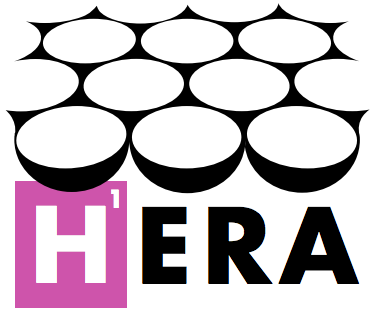
\includegraphics[width=15cm]{HERA.png} % Logo or a photo of you, adjust its dimensions here
%\end{minipage}
%\hspace{2cm}
%\begin{minipage}[b]{0.15\linewidth}
%\Huge{\textbf{PAPER}}
%\end{minipage}
%\hspace{2cm}
%\begin{minipage}[b]{0.15\linewidth}
%\Huge{\textbf{MWA}}
%\end{minipage}

%
%\begin{minipage}[b]{0.25\linewidth}
%\color{DarkSlateGray}\Large \textbf{Contact Information:}\\
%Physics\\ % Address
%Brown University\\
%$\#$ George St., Providence, RI\\\\
%Phone: +1 (000) 111 1111\\ % Phone number
%Email: \texttt{Add Emails}\\ % Email address
%\end{minipage}
%
% Maybe we don't need the Brown logo, consider replacing with PAPER,HERA,MWA logos?


%\vspace{1cm} % A bit of extra whitespace between the header and poster content

%----------------------------------------------------------------------------------------

\begin{multicols}{4} % This is how many columns your poster will be broken into, a poster with many figures may benefit from less columns whereas a text-heavy poster benefits from more

%----------------------------------------------------------------------------------------
%	ABSTRACT
%----------------------------------------------------------------------------------------

%\color{Navy} % Navy color for the abstract

%\begin{abstract}

%Following the recombination of hydrogen and release of the cosmic microwave background radiation at redshift $z \sim 1100$, the baryonic matter of the universe consisted mostly of neutral hydrogen and helium. Gradually, small inhomogeneities collapsed and ignited the first luminous structures. Energetic photons emitted from the first stars and quasars reionized the surrounding medium, producing ionized bubbles which grew and merged into the fully ionized intergalactic medium we see today. This \emph{Epoch of Reionization} (EoR) remains a poorly-understood period of the universe's history which offers a wealth of cosmological and astrophysical information.

%The Pober lab is part of an international effort to build instruments capable of studying the EoR. The neutral hydrogen (HI) of the EoR emits faintly at a wavelength of 21cm, due to the hyperfine transition. This emission is unique to neutral hydrogen, and is anti-correlated with the ionized (HII) regions that fill the universe through the EoR. CMB constraints and quasar absorption spectra put the EoR as occurring within the redshift range $6 < z < 12$, which means 21cm emissions will redshift to meter scale wavelengths. This is accessible to modern radio interferometers, including the \emph{Donald C. Backer Precision Array for Probing the Epoch of Reionization} (PAPER), the \emph{Murchison Widefield Array} (MWA), and the recently-funded \emph{Hydrogen Epoch of Reionization Array} (HERA).

%The main focus of the Pober Lab is the direct observation of the 21cm Neutral Hydrogen (HI) emission through the use of radio telescope arrays to detect the signal from the Epoch of Reionization (EoR). The 21cm hyperfine spin flip, which is typically a forbidden transition, has a mean lifetime on the order of 100 million years. This time scale, and the abundance of HI in the universe gives us the ability to map the progress of reionization which has the redshift range of 6 $<$ z $<$ 12. To observe the reionization of the HI, we use radio telescope arrays, because the 21cm emission corresponds to 1420 MHz at rest and when received at Earth corresponds to 100-200 MHz due to cosmological redshifting. The Pober Lab contributes to several international radio telescope array collaborations which include the Precision Array for Probing the Epoch of Reionization (PAPER), the Murchison Widefield Array (MWA) and the newly NSF funded Hydrogen Epoch of Reionization Array (HERA).

%\end{abstract}

%----------------------------------------------------------------------------------------
%	INTRODUCTION
%----------------------------------------------------------------------------------------
\color{DarkSlateGray}  % SaddleBrown color for the introduction

\section*{Introduction}
Following the recombination of hydrogen and release of the cosmic microwave background radiation at redshift $z \sim 1100$, the baryonic matter of the universe consisted mostly of neutral hydrogen and helium. Gradually, small inhomogeneities collapsed and ignited the first luminous structures. Energetic photons emitted from the first stars and quasars reionized the surrounding medium, producing ionized bubbles which grew and merged into the fully ionized intergalactic medium we see today. This \emph{Epoch of Reionization} (EoR) remains a poorly-understood period of the universe's history which offers a wealth of cosmological and astrophysical information.

The Pober lab is part of an international effort to build instruments capable of studying the EoR. The neutral hydrogen (HI) of the EoR emits faintly at a wavelength of 21cm, due to the hyperfine transition. This emission is unique to neutral hydrogen, and is anti-correlated with the ionized (HII) regions that fill the universe through the EoR. CMB constraints and quasar absorption spectra put the EoR as occurring within the redshift range $6 < z < 12$, which means 21cm emissions will redshift to meter scale wavelengths. This is accessible to modern radio interferometers, including the \emph{Donald C. Backer Precision Array for Probing the Epoch of Reionization} (PAPER), the \emph{Murchison Widefield Array} (MWA), and the recently-funded \emph{Hydrogen Epoch of Reionization Array} (HERA).

\begin{figure}[H]
\centering
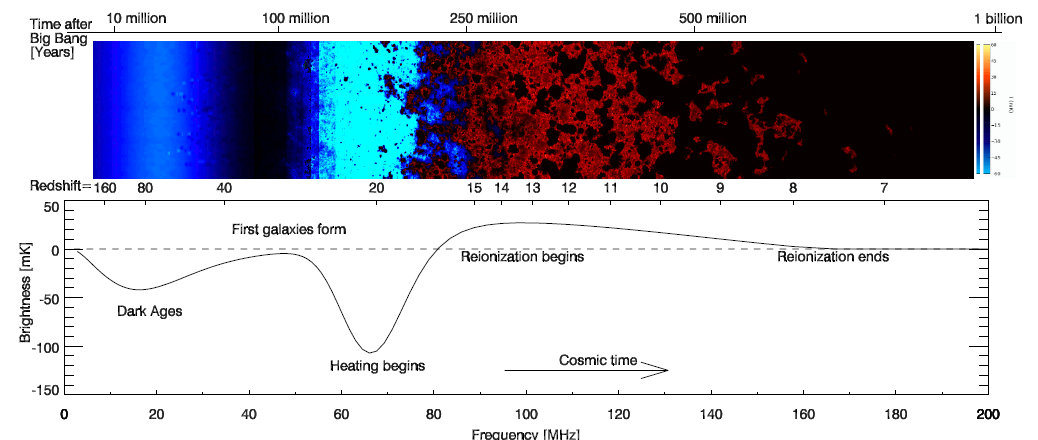
\includegraphics[width=1.0\linewidth]{figures/global_history.png}
\caption{The global differential brightness temperature, $\delta T_b$, evolution over redshift 6 $<$ z $<$ 160. $\delta T_b$ becomes observable when 
the spin temperature $T_S$ decouples from the CMB temperature, $T_{CMB}$ through the Wouthyusen-Field effect, this can be seen in 
Eqn. \ref{difftemp}}.
\end{figure}


\subsubsection*{Differential Brightness Temperature}
\begin{equation}
\label{difftemp}
\resizebox{.9\hsize}{!}{$
\delta T_{b} = 28mK(1+\delta)x_{HI}\Big(1-\frac{T_{CMB}}{T_{spin}}\Big)\Big(\frac{\Omega_{b}h^2}{0.0223}\Big)\sqrt{\Big(\frac{1+z}{10}\Big)\Big(\frac{0.24}{\Omega_m}\Big)}\Big[ \frac{H(z)/(1+z)}{dv_{||}/dr_{||}}\Big]$}
\end{equation}
The differential brightness temperature describes the complex nature of the neutral hydrogen spin temperature,$T_S$ decoupling from the CMB background temperature $T_{CMB}$, the neutral fraction of Hydrogen, $x_{HI}$, and the mass density contrast, $\delta$.
$\delta T_b$ also describes an important relationship between cosmological and astrophysical parameters, showing that measuring what is seen as a cosmological epoch has astrophysical relevance.


%----------------------------------------------------------------------------------------
%	OBJECTIVES
%----------------------------------------------------------------------------------------
% DarkSlateGray color for the rest of the content
\section*{The Foreground Problem} %[I dont need all of these plots, they're just there to be cut as needed or if necessary to take up more space]
Galactic and extragalactic foregrounds pose a difficult problem when trying to measure the 21cm EoR signal. Relative to galactic foregrounds, the EoR signal is $\sim$ 5 orders of magnitude smaller than the galactic emissions that exist between our observing radio telescope arrays and the highly redshifted 21cm signal. The overlapping sources of power in our observations can be seen in Fig. \ref{fig:foregroundsrcs}.


\begin{figure}[H]
\centering
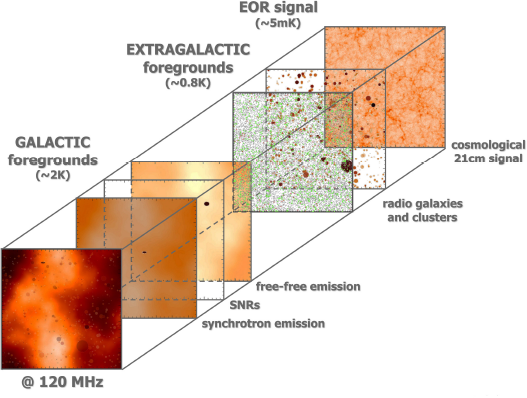
\includegraphics[width=0.55\linewidth]{figures/foreground_figure.png}
\caption{The various cosmological and galactic sources that contribute to the measured sky temperature, and their relative strengths. \textbf{Source}: Saleem Zaroubi, \textit{https://ned.ipac.caltech.edu/level5/March14/Zaroubi/Zaroubi5.html}}\label{fig:foregroundsrcs}
\end{figure}
To overcome foreground dominance in our power spectrum analysis we can use a combination of foreground power mitigating techniques as outlined in the following subsections.
%The issue of foreground emission dominance in our power spectrum can be overcome through the mixed use of the following traditional and novel foreground mitigation techniques. \\
\subsubsection*{Foreground Subtraction}
Foreground subtraction is performed in the image domain using an extragalactic source catalog. The source catalog is used to generate a foreground model which can then be fit by an $n^{th}$ order polynomial and subtracted from the observation.
%Baseline visibilities are gridded to form an image which is calibrated to a catalog model. The catalog model contains point sources from 
%surveys which contain the sources' right ascension, declination, and flux in stokes I. The model built from the catalog of sources is 
%additionally convolved with the telescope arrays synthesized beam model. The resulting model which has been built can then be subtracted 
%from the observation leaving behind the EoR signal and diffuse emissions.
\begin{figure}[H]
\centering
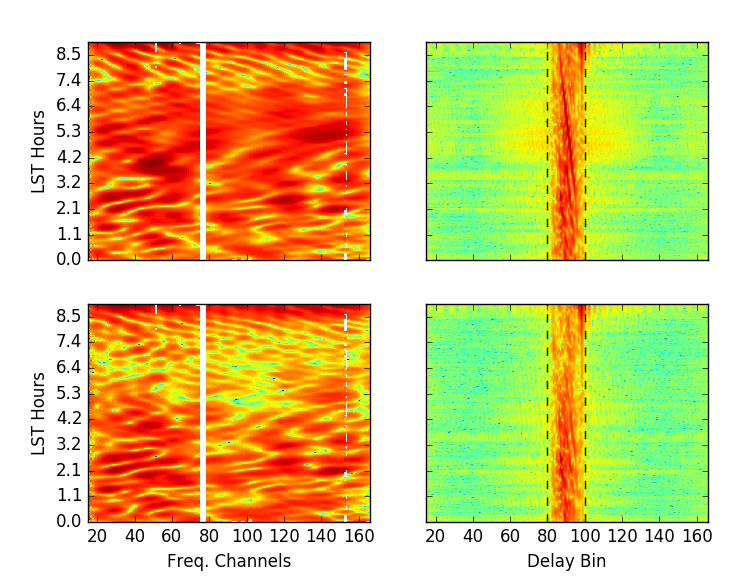
\includegraphics[width=0.6\linewidth]{figures/foresub.png}
\caption{LST binned visibility of a 30m East-West baseline from the PAPER-64 array. The left plots show a baseline visibility pre- and post subtraction. The right plots show the delay transform of the left plots, demonstrating the foreground power being concentrated within the horizon limit (dotted lines).}
\label{foregroundsrcs1}
\end{figure}


\subsubsection*{Foreground Avoidance}
\begin{equation}
\label{delaytransform}
V_b(\tau) = \int dl dm d\nu A(l,m,\nu)I(l,m,\nu)e^{-2\pi i\nu(\tau_g -\tau)}
\end{equation}
Equation \ref{delaytransform} demonstrates the delay transform used to transform a visibility to delay space. By working in delay space it can be seen in both Figs. \ref{foregroundsrcs1} \& \ref{foregroundsrcs2} that power from foreground sources are confined within a delay limit known as the horizon limit.

%Taking the Fourier transform of a baseline visibility over frequency with the geometric group delay offset (eqn. \ref{delaytransform}) results %in smooth spectrum foregrounds bunching up nearest to the delay of $\tau = 0$. This is because foreground sources have a maximal %geometric delay associated with a baseline length, $|\vec{b}|$, which is also known as the horizon limit. The EoR signal is unsmooth %spectrally, distinguishing it from foreground sources, and pushing it beyond the horizon limit imposed by the baseline length. Using this %information, delays below the horizon limit can be filtered giving significant foreground power removal.

\begin{figure}[H]
\centering
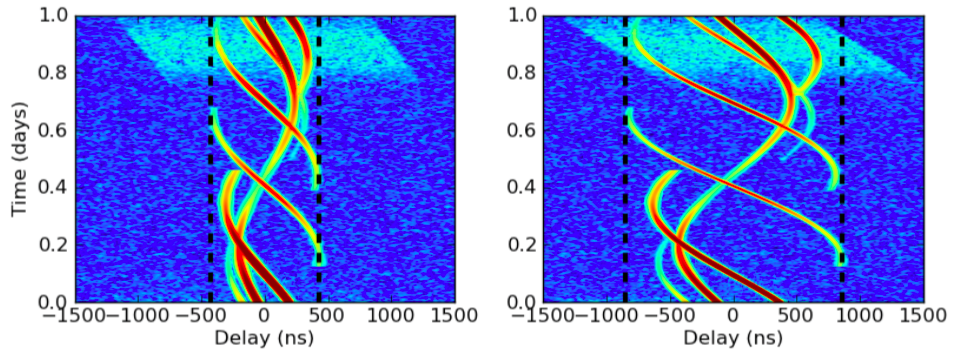
\includegraphics[width=0.8\linewidth]{figures/delaytransform.png}
\caption{Delay transform visibilities of two different baseline types. Smooth spectral sources moving between delays over time can be seen to remain within the horizon limit (dotted), while unsmooth spectral sources (light blue) extend beyond the horizon limit.  \textbf{Source}: Aaron Parsons, \textit{A Per Baseline Delay-Spectrum Technique for Accessing the 21cm Cosmic Reionization Signature, Apj. 2012}}
\label{foregroundsrcs2}
\end{figure}

%----------------------------------------------------------------------------------------
%	MATERIALS AND METHODS
%----------------------------------------------------------------------------------------


\section*{Calibration}

The most common techniques we use on visibility calibration are redundant calibration and sky model based calibration. Sky model calibration requires some preknowledges about the sky. With our assumptions about source structures of the sky and understanding of our instrument, we use FHD (Fast Holographic Deconvolution) to calibrate visibility data. The algorithm FHD uses is basically 'CLEAN' algorithm. Redundant calibration is sky model independent. All it assumes is that same antenna separations should measure exact the same Fourier mode of the sky. Redundant calibration requires antenna array with good redundant calibratability, like PAPER64, MWA PhaseII hexes and HERA.

\begin{figure}[H]
\centering
\label{Redundant calibration on MWA PhaseII ORBCOMM data}
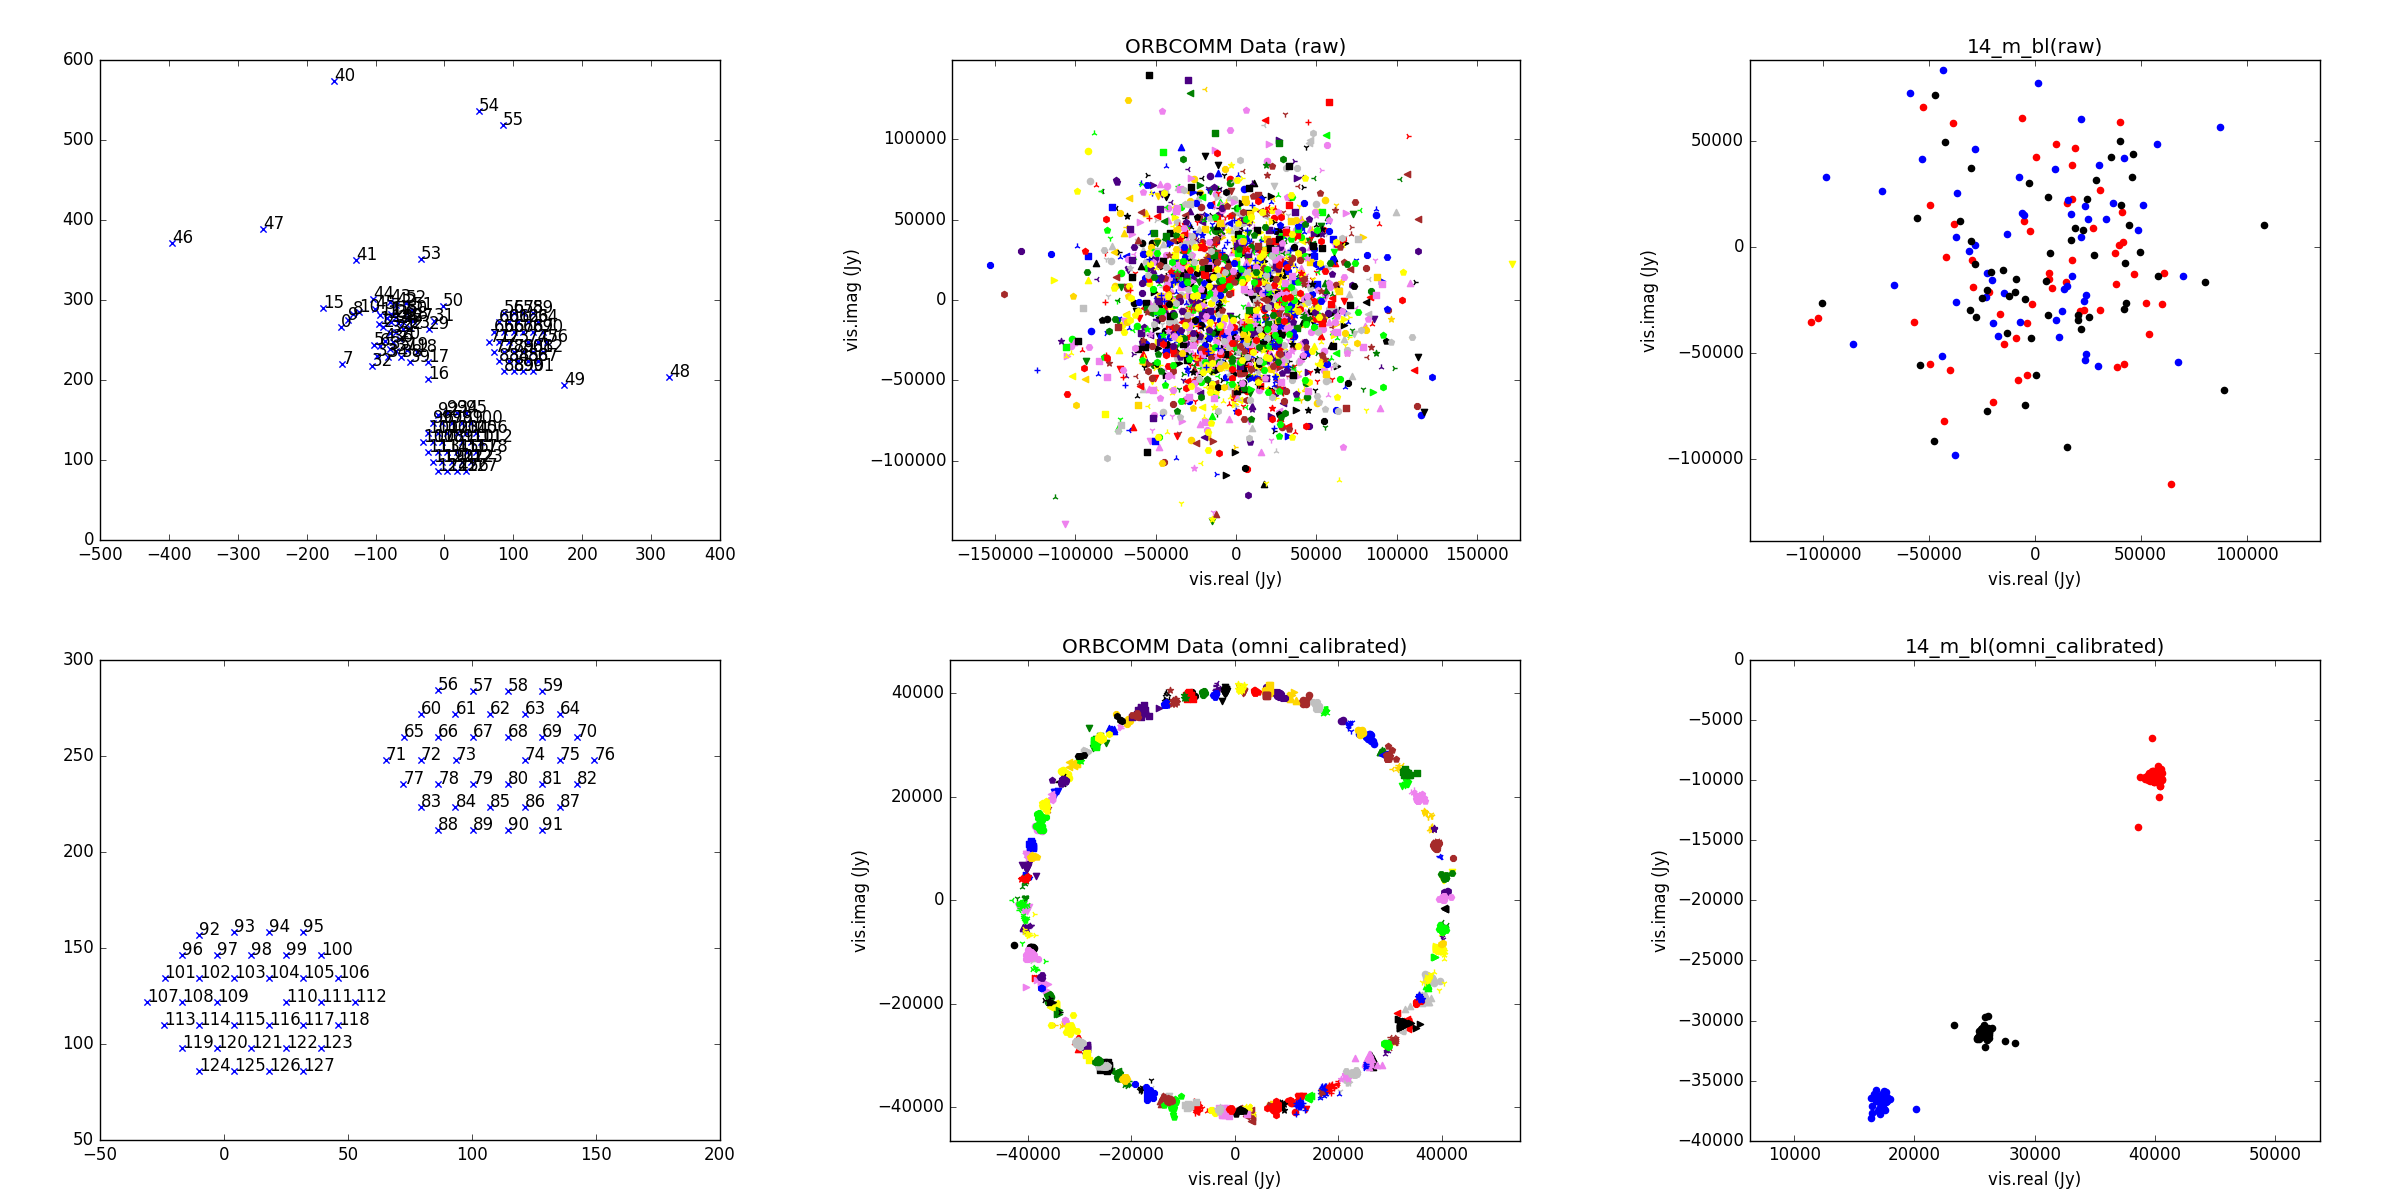
\includegraphics[width=0.85\linewidth]{figures/omnical_on_ORBCOMM.png}
\caption{Top left: MWA PhaseII configuration. Bottom left: Zoom in into PhaseII hexes. Middle top: raw ORBCOMM complex visibility data at 137.1MHz. Each combination of color and shape stands for data from a unique type of baseline. Middle bottom: ORBCOMM data after redundant calibration. Right top: raw 14m baseline data. Right bottom: calibrated 14m baseline data.}
\end{figure}


%----------------------------------------------------------------------------------------
\section*{Simulation}

The particular characteristics of an array can introduce unexpected effects into the data. To detect a signal as weak as the EoR, understanding and mitigating instrumental effects is critical. For this reason, much effort has been put into simulating the full analysis pipeline, from the point and diffuse sources on the sky to the raw visibilities that come out to the power spectrum estimations.

Fast Holographic Deconvolution (FHD) is a purpose-built software framework for analyzing MWA data. FHD does foreground subtraction by \emph{forward modeling}, which builds a simulated data set, including instrumental effects, and subtracts it from the actual data. This forward modeling feature can also be used as a standalone simulation tool, to generate raw visibilities of foregrounds, noise, and EoR off of existing and future 21cm experiments.
\begin{figure}[H]
\centering
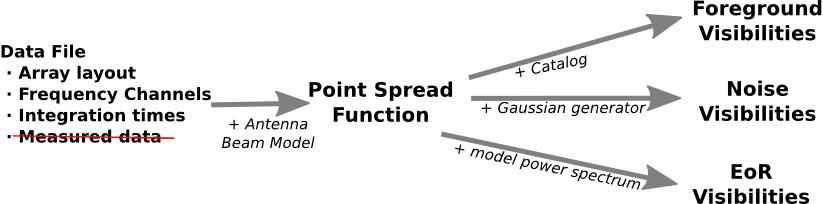
\includegraphics[scale=1]{figures/sim_flowchart.png}
\caption{A sample data file (or generated data file) holds array coordinates over time and the frequency channels of the instrument. Given a beam model for the antenna, FHD calculates the full synthesized beam (or point-spread function) for a particular time and set of frequencies. The synthesized beam can then convert a sky catalog into a set of foreground visibilities for the instrument. External EoR simulations can also be fed in to test EoR sensitivity, or Gaussian noise can be injected to simulate noise.}
\end{figure}

%------------------------------------------------
%	RESULTS 
%----------------------------------------------------------------------------------------

\section*{Radio Telescope Arrays}
\begin{figure}[H]
\centering
\label{fig:PAPER}
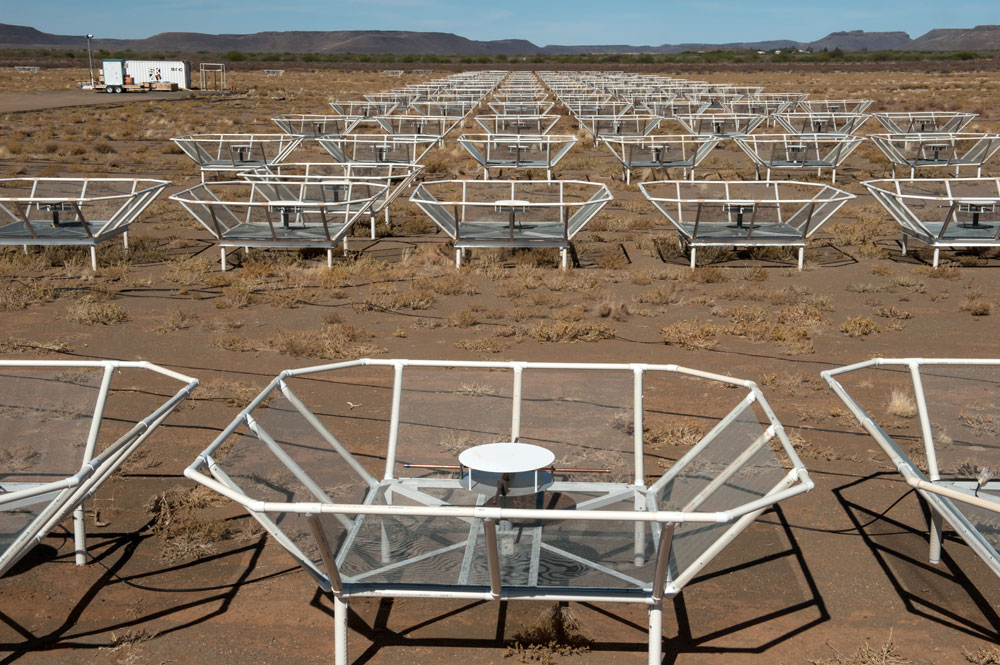
\includegraphics[width=0.8\linewidth]{figures/paper}
\caption{PAPER - Located in South Africa in the Karoo desert, consists of 128 dipole antennas and is considered a $1^{st}$ generation radio telescope array. PAPER is a redundant array configuration, which means it redundantly probes many of the same $k_\perp$ modes and allows for the use of redundant calibration.}
\end{figure}

\begin{figure}[H]
\centering
\label{fig:MWA}
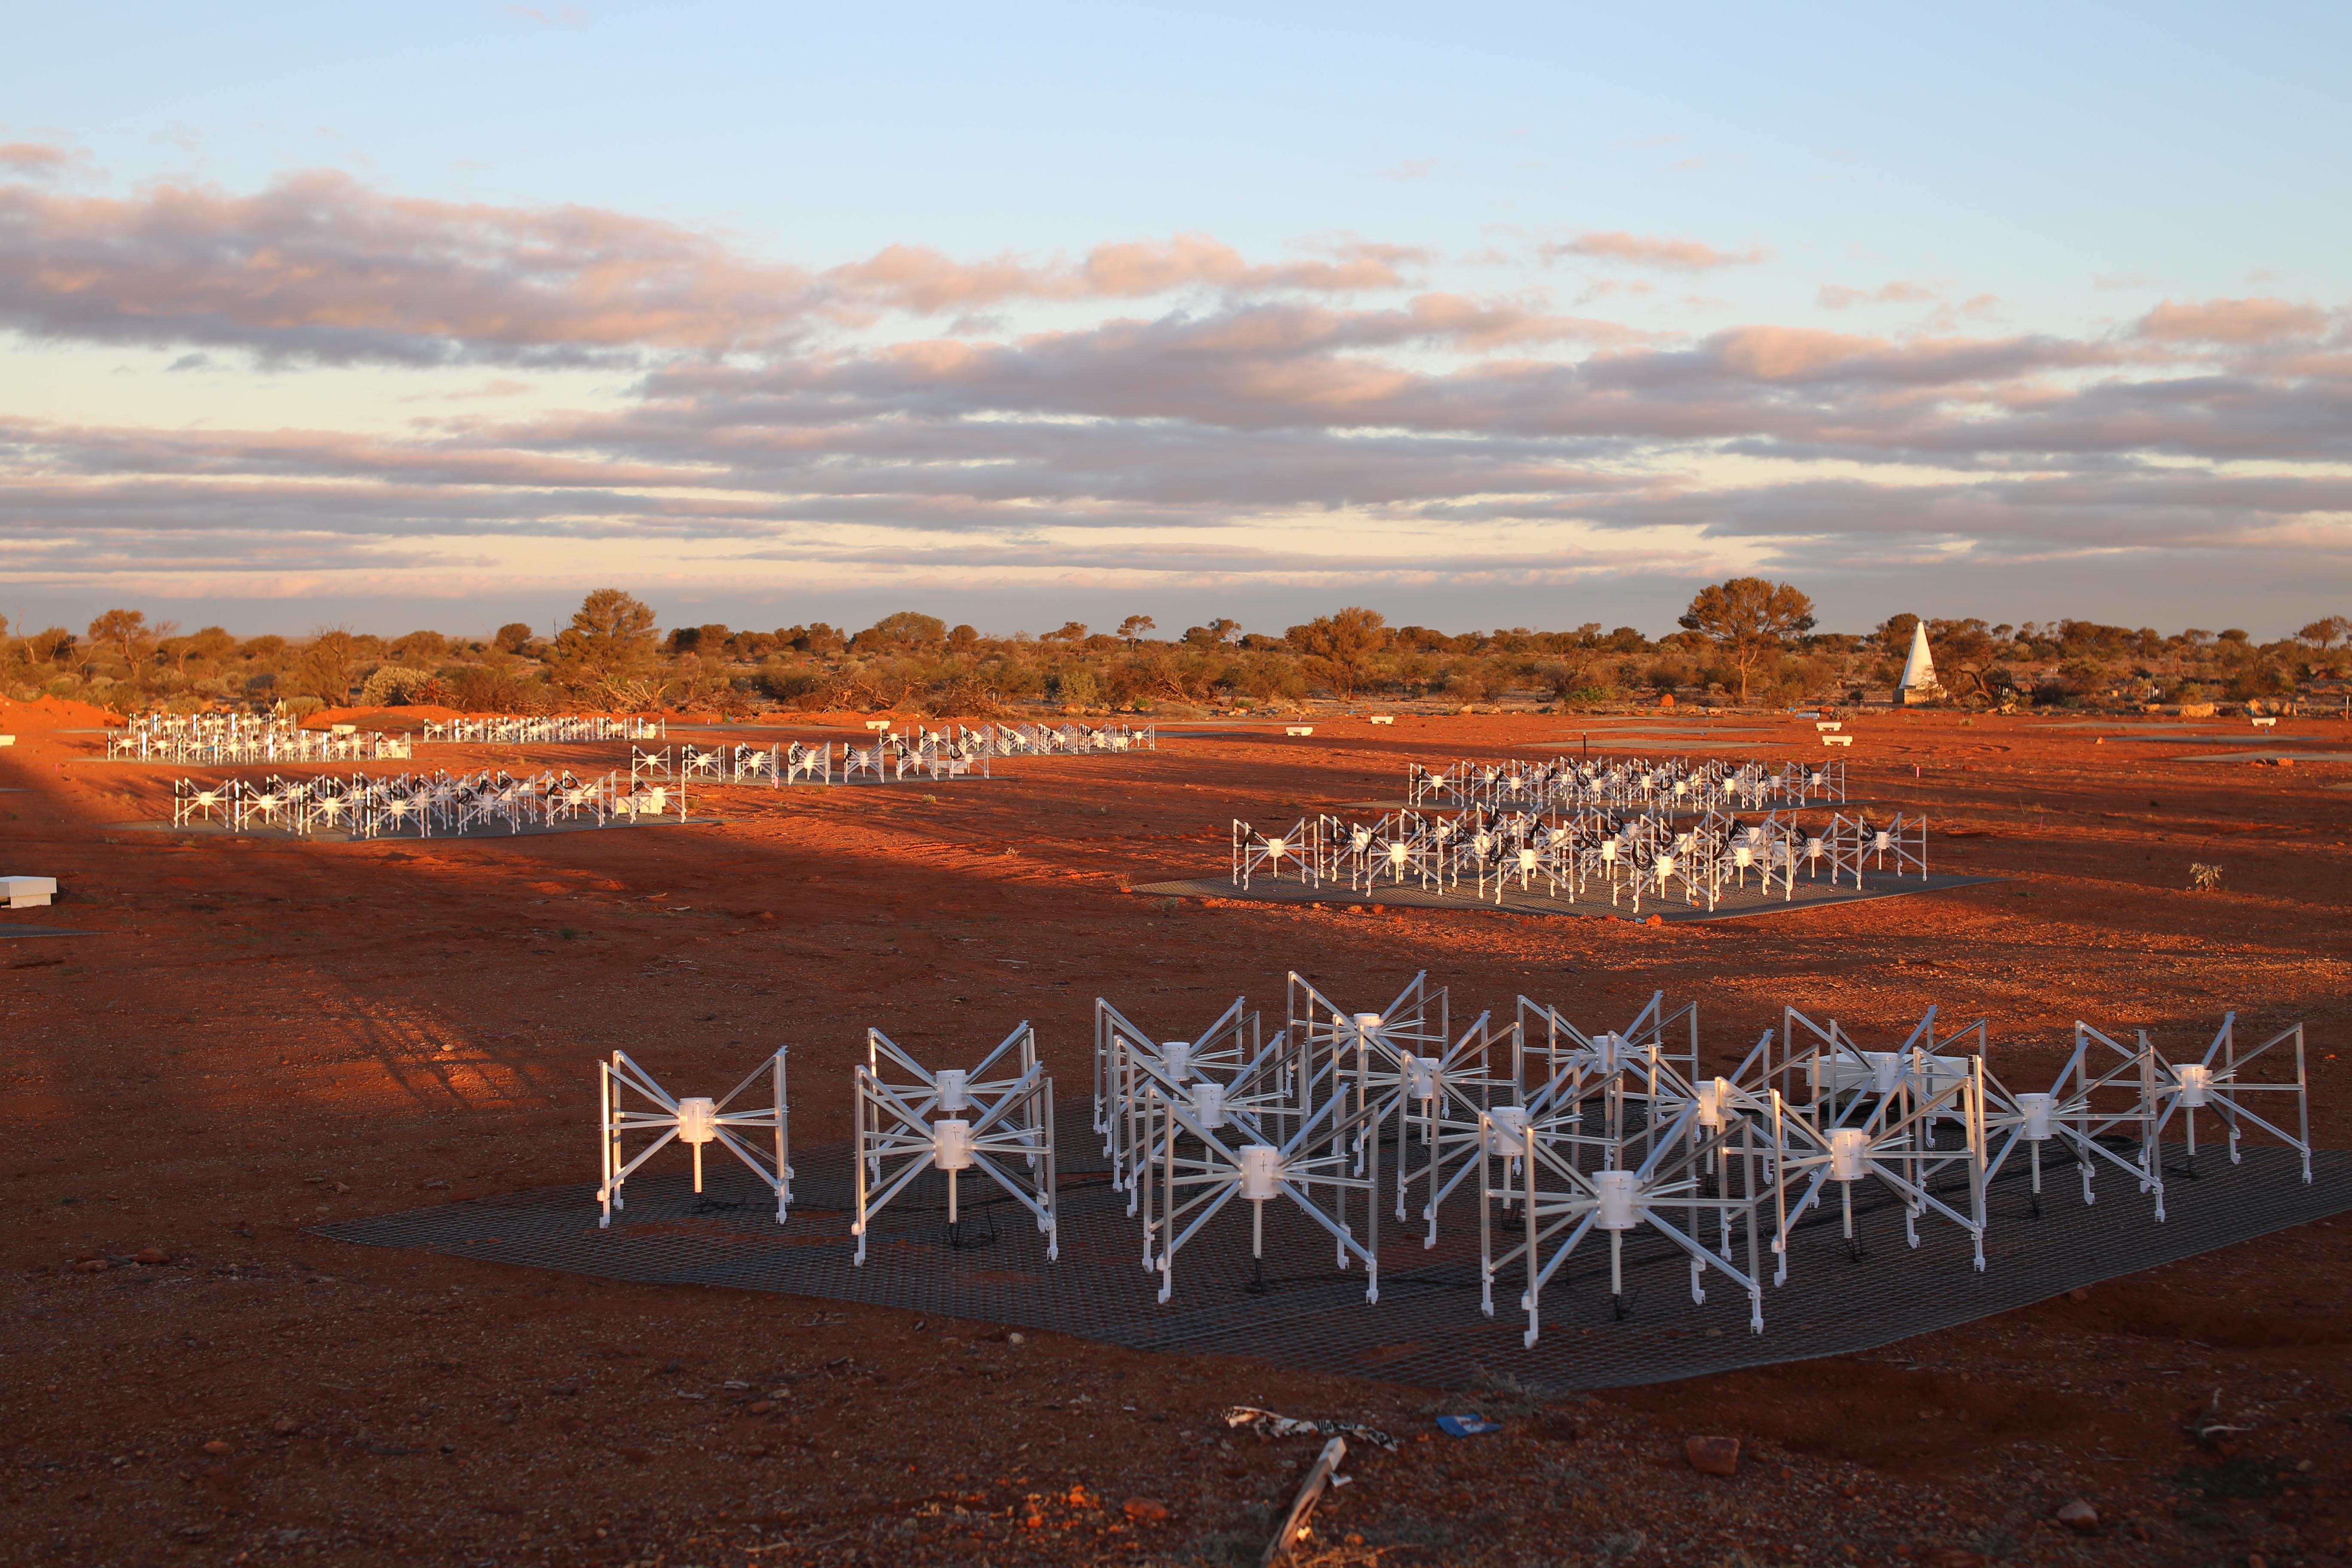
\includegraphics[width=0.8\linewidth]{figures/phaseII_tiles.jpg}
\caption{MWA - Located in Western Australia in the Murchison Radio Astronomy Observatory. The MWA is a multipurpose array that is used for additional observations such as ionosphere studies and transient radio signals. It consists of 128 tiles which are each made up of 16 dipole antennae.The MWA array configuration is maximized for uv coverage which improves the imaging capability of the array. MWA is a pathfinder project for the Square Kilometer Array (SKA).}
\end{figure}

\begin{figure}[H]
\centering
\label{fig:HERA}
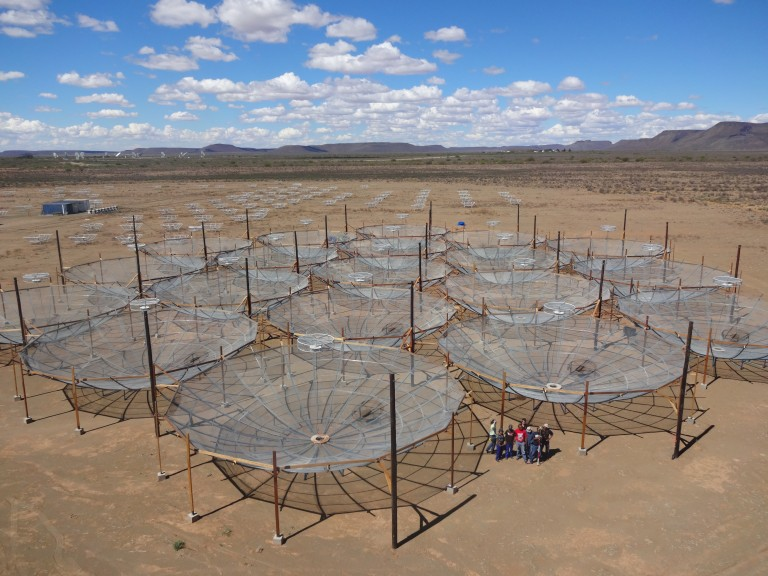
\includegraphics[width=0.8\linewidth]{figures/HERA19.png}
\caption{HERA - Located at the same site as PAPER in the Karoo desert. The current phase of HERA consists of 19 14m parabolic dishes. HERA is also a pathfinder project for the SKA.}
\end{figure}

%----------------------------------------------------------------------------------------
%	CONCLUSIONS
%----------------------------------------------------------------------------------------

%\color{SaddleBrown} % SaddleBrown color for the conclusions to make them stand out

%\section*{Conclusions}

%[Do we have conclusions?] [No?]


\color{DarkSlateGray} % Set the color back to DarkSlateGray for the rest of the content

%----------------------------------------------------------------------------------------
%	FORTHCOMING RESEARCH
%----------------------------------------------------------------------------------------

%\section*{Forthcoming Research}
%Probably not necessary because we can just add a blurb in the Radio Telescope arrays section about HERA?
%[Picture of HERA-331?]


 %----------------------------------------------------------------------------------------
%	REFERENCES
%----------------------------------------------------------------------------------------
% We referenced all the best people
%\nocite{*} % Print all references regardless of whether they were cited in the poster or not
%\bibliographystyle{plain} % Plain referencing style
%\bibliography{sample} % Use the example bibliography file sample.bib

%----------------------------------------------------------------------------------------
%	ACKNOWLEDGEMENTS
%----------------------------------------------------------------------------------------

%\section*{Acknowledgements}
%I refuse to acknowledge anyone or any thing!!!!!!!


%----------------------------------------------------------------------------------------
\end{multicols}
%\begin{minipage}[b]{0.19\linewidth}
%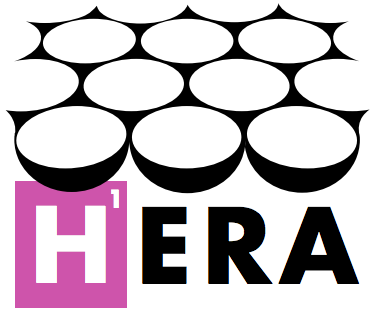
\includegraphics[width=15cm]{HERA.png} % Logo or a photo of you, adjust its dimensions here
%\end{minipage}
%\hspace{2cm}
%\begin{minipage}[b]{0.25\linewidth}
%\Huge{\textbf{PAPER}}
%\end{minipage}
%\hspace{2cm}
%\begin{minipage}[b]{0.25\linewidth}
%\Huge{\textbf{MWA}}
%\end{minipage}
\end{document}
